\documentclass[11pt,letterpaper]{article}
\textwidth 6.5in
\textheight 9.in
\oddsidemargin 0in
\headheight 0in
\usepackage{graphicx}
\usepackage{fancybox}
\usepackage[utf8]{inputenc}
\usepackage{epsfig,graphicx}
\usepackage{multicol,pst-plot}
\usepackage{pstricks}
\usepackage{amsmath}
\usepackage{amsfonts}
\usepackage{amssymb}
\usepackage{eucal}
\usepackage{subfigure}
\usepackage{enumitem}
\usepackage{hyperref}
\usepackage[left=2cm,right=2cm,top=2cm,bottom=2cm]{geometry}
\pagestyle{empty}
\DeclareMathOperator{\tr}{Tr}
\newcommand*{\op}[1]{\check{\mathbf#1}}
\newcommand{\Mod}[1]{\ (\mathrm{mod}\ #1)}
\newcommand{\bra}[1]{\langle #1 |}
\newcommand{\ket}[1]{| #1 \rangle}
\newcommand{\braket}[2]{\langle #1 | #2 \rangle}
\newcommand{\mean}[1]{\langle #1 \rangle}
\newcommand{\opvec}[1]{\check{\vec #1}}
\newcommand{\bb}[1]{\mathbb{#1}}
\newcommand{\suchthat}{\;\ifnum\currentgrouptype=16 \middle\fi|\;}
\usepackage{lipsum}

\usepackage{listings}
\usepackage{color}

\definecolor{codegreen}{rgb}{0,0.6,0}
\definecolor{codegray}{rgb}{0.5,0.5,0.5}
\definecolor{codepurple}{rgb}{0.58,0,0.82}
\definecolor{backcolour}{rgb}{0.95,0.95,0.92}

\lstdefinestyle{mystyle}{
	backgroundcolor=\color{backcolour},   
	commentstyle=\color{codegreen},
	keywordstyle=\color{magenta},
	numberstyle=\tiny\color{codegray},
	stringstyle=\color{codepurple},
	basicstyle=\footnotesize,
	breakatwhitespace=false,         
	breaklines=true,                 
	captionpos=b,                    
	keepspaces=true,                 
	numbers=left,                    
	numbersep=5pt,                  
	showspaces=false,                
	showstringspaces=false,
	showtabs=false,                  
	tabsize=2
}

\lstset{style=mystyle}

\begin{document}
\pagestyle{plain}

\begin{flushleft}
Name: Awies Mohammad Mulla\\
UCSD PID: A59016119
\end{flushleft}

\begin{flushright}\vspace{-15mm}

\includegraphics[height=2cm]{logo.png}
\end{flushright}
 
\begin{center}\vspace{-1cm}
\textbf{\large ECE 269 Linear Algebra and Applications}\\
\textbf{\large Mini Project 3}\\
\end{center}

 
\rule{\linewidth}{0.1mm}

\section*{Problem 1}
\subsection*{Ten most representative Eigenfaces (Neutral)}
% insert 10 images here in a compact but visible form
\begin{figure}[htbp]
    \centering
    \subfigure{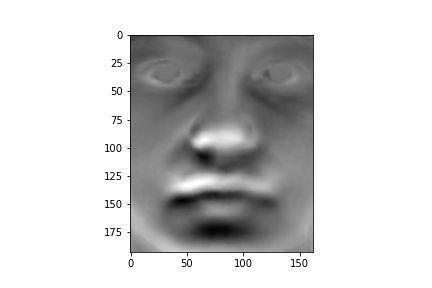
\includegraphics[width=0.25\textwidth]{../outputs/ans1/neutral_eigenface_0.png}}
    \subfigure{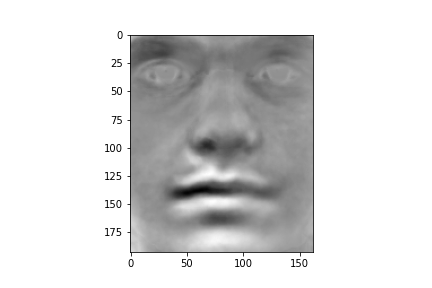
\includegraphics[width=0.25\textwidth]{../outputs/ans1/neutral_eigenface_1.png}}\\
    \subfigure{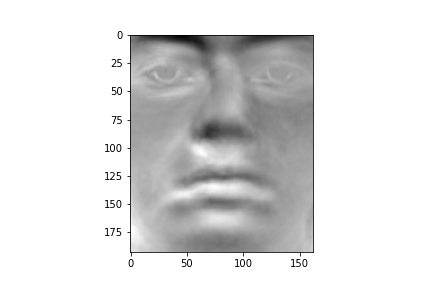
\includegraphics[width=0.25\textwidth]{../outputs/ans1/neutral_eigenface_2.png}}
    \subfigure{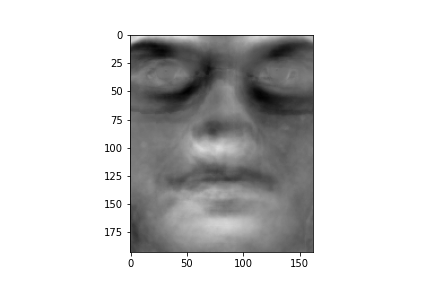
\includegraphics[width=0.25\textwidth]{../outputs/ans1/neutral_eigenface_3.png}}\\
    \subfigure{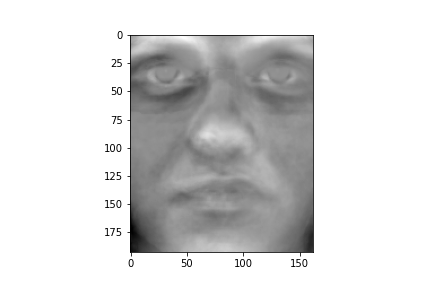
\includegraphics[width=0.25\textwidth]{../outputs/ans1/neutral_eigenface_4.png}}
    \subfigure{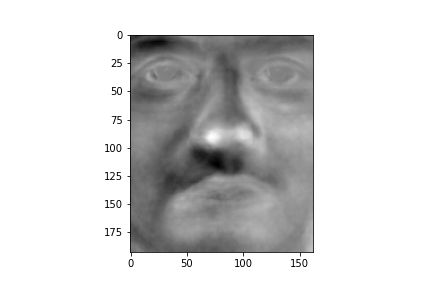
\includegraphics[width=0.25\textwidth]{../outputs/ans1/neutral_eigenface_5.png}}\\
    \subfigure{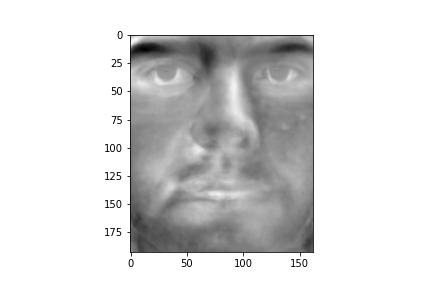
\includegraphics[width=0.25\textwidth]{../outputs/ans1/neutral_eigenface_6.png}}
    \subfigure{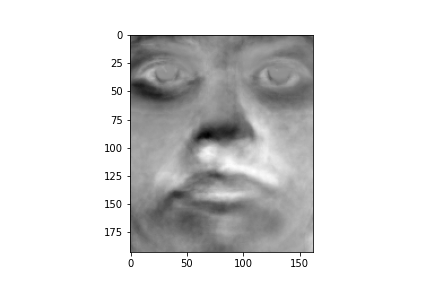
\includegraphics[width=0.25\textwidth]{../outputs/ans1/neutral_eigenface_7.png}}\\
    \subfigure{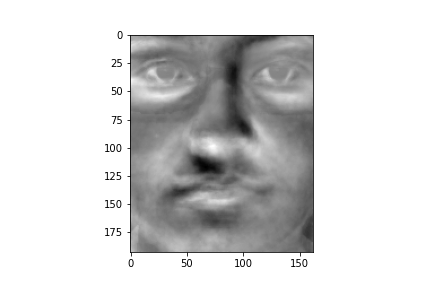
\includegraphics[width=0.25\textwidth]{../outputs/ans1/neutral_eigenface_8.png}}
    \subfigure{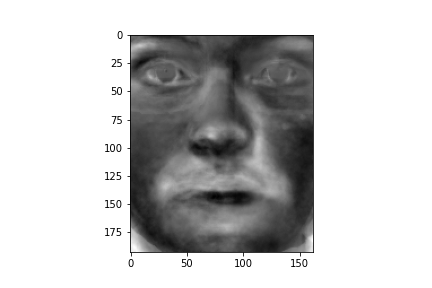
\includegraphics[width=0.25\textwidth]{../outputs/ans1/neutral_eigenface_9.png}}\\
    \caption{Ten most representative Eigenfaces (Top left to bottom right)}
    \end{figure}
\subsection*{Ten most representative Eigenfaces (Smile)}
% insert 10 images here in a compact but visible form
\begin{figure}[htbp]
    \centering
    \subfigure{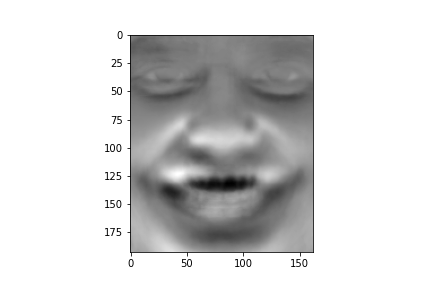
\includegraphics[width=0.25\textwidth]{../outputs/ans1/smile_eigenface_0.png}}
    \subfigure{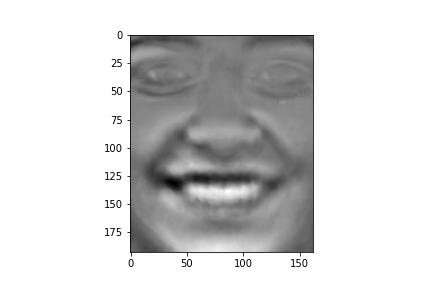
\includegraphics[width=0.25\textwidth]{../outputs/ans1/smile_eigenface_1.png}}\\
    \subfigure{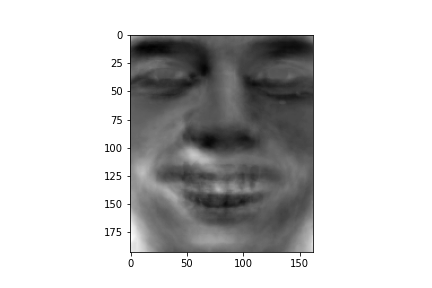
\includegraphics[width=0.25\textwidth]{../outputs/ans1/smile_eigenface_2.png}}
    \subfigure{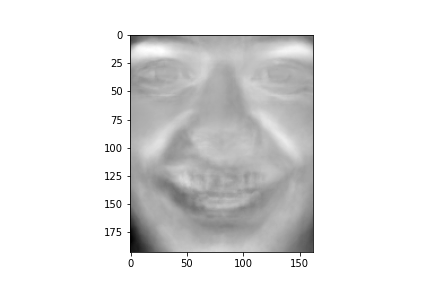
\includegraphics[width=0.25\textwidth]{../outputs/ans1/smile_eigenface_3.png}}\\
    \subfigure{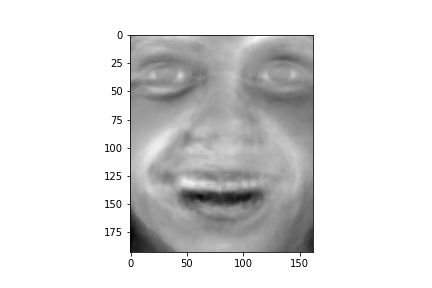
\includegraphics[width=0.25\textwidth]{../outputs/ans1/smile_eigenface_4.png}}
    \subfigure{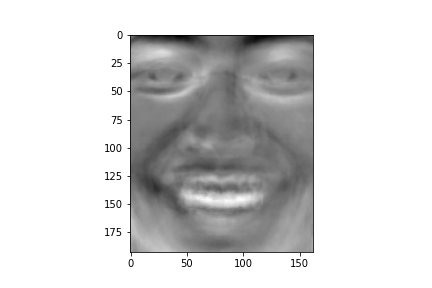
\includegraphics[width=0.25\textwidth]{../outputs/ans1/smile_eigenface_5.png}}\\
    \subfigure{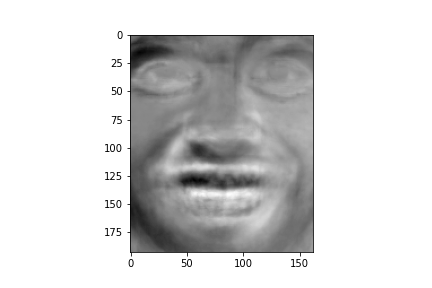
\includegraphics[width=0.25\textwidth]{../outputs/ans1/smile_eigenface_6.png}}
    \subfigure{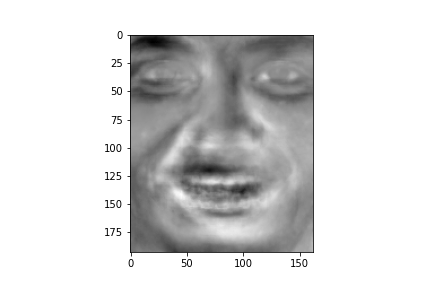
\includegraphics[width=0.25\textwidth]{../outputs/ans1/smile_eigenface_7.png}}\\
    \subfigure{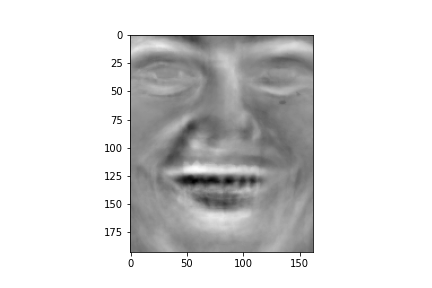
\includegraphics[width=0.25\textwidth]{../outputs/ans1/smile_eigenface_8.png}}
    \subfigure{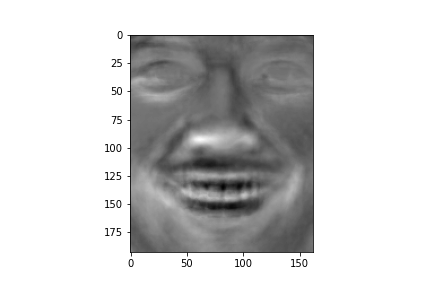
\includegraphics[width=0.25\textwidth]{../outputs/ans1/smile_eigenface_9.png}}\\
    \caption{Ten most representative Eigenfaces (Top left to bottom right)}
    \end{figure}
\subsection*{Plots and Analysis}
\begin{enumerate}
    \item  Plot of normalised eigenvalues is shown below. From this plot, we can infer that we get relevant features only from eigenfaces (Principal Components) generated from eigenvectors corresponding to largest 25 eigenvalues. As the effective weights of other eigenvectors is almost negligible i.e. they could not improve the representation by an appreciable factor. Hence, we chose 25 principal components.
    \item  Plot shown below represents singular values of the data matrix. Singular values ($\sigma_i$) can be represented in terms of eigenvalues ($\lambda_i$) as $\sigma_i \ = \ \sqrt{\lambda_i}$. Hence, this plot can also be used to give above inference and choose appropriate number of principal components.
\end{enumerate}
\begin{figure}[htbp]
    \centering
    \subfigure[Normalised Eigenvalues for Neutral Faces]{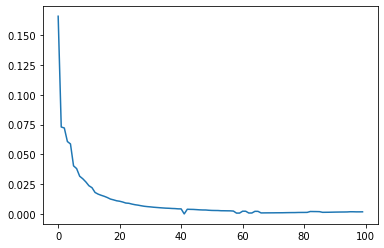
\includegraphics[width=0.4\textwidth]{../outputs/ans1/neutral_normalised_eigenvalues.png}}
    \subfigure[Normalised Eigenvalues for Smile Faces]{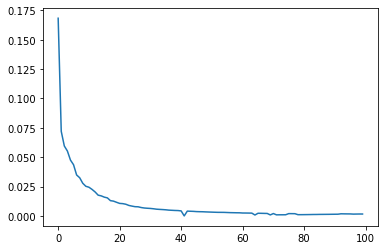
\includegraphics[width=0.4\textwidth]{../outputs/ans1/smile_normalised_eigenvalues.png}} \\
    \subfigure[Singular Values for Neutral Faces]{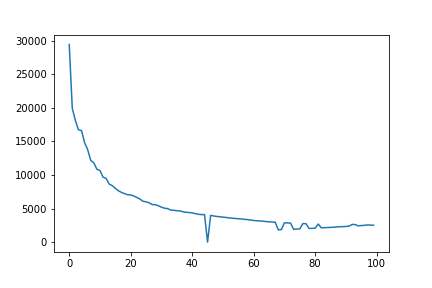
\includegraphics[width=0.4\textwidth]{../outputs/ans1/neutral_singular_values.png}}
    \subfigure[Singular Values for Smile Faces]{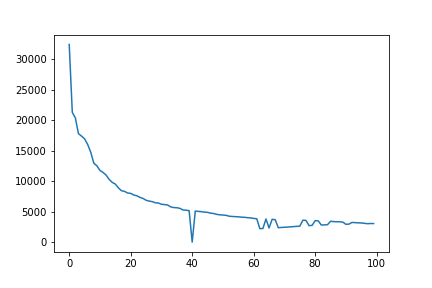
\includegraphics[width=0.4\textwidth]{../outputs/ans1/smile_singular_values.png}} \\
\end{figure}
\section*{Problem 2}
\begin{figure}[htbp]
    \centering
    \subfigure[MSE vs Number of PCs]{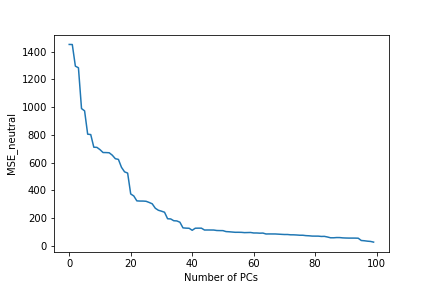
\includegraphics[width=0.50\textwidth]{../outputs/ans2/MSE_neutral.png}}
    \end{figure}
\begin{enumerate}
    [label=$\bullet$]
    \item As we can see from the plot, initially MSE decreases drastically when we increase the number of PCs. After a certain number of PCs, the decrease in MSE is not so steep eventhough we increase the number of PCs. This is due to similar reason mentioned in the previous part. 
    \item The Principal Components, after about 25 most representative eigenfaces, does not provide substantial additional information to improve the reconstructed image drastically. This was also inferred by analysing corresponding eigenvalues in problem 1. 
\end{enumerate}
\begin{figure}[htbp]
    \centering
    \subfigure[5 PCs]{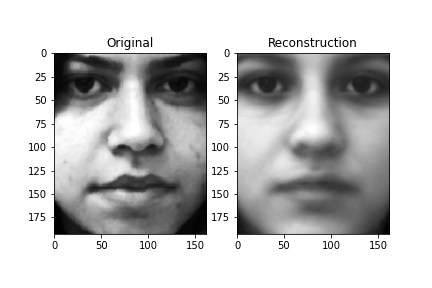
\includegraphics[width=0.40\textwidth]{../outputs/ans2/PCs_5.png}}
    \subfigure[10 PCs]{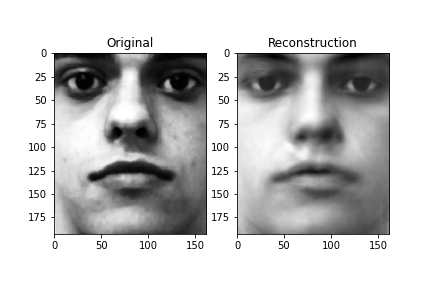
\includegraphics[width=0.40\textwidth]{../outputs/ans2/PCs_10.png}} \\
    \end{figure}
\begin{figure}
    \centering
    \subfigure[15 PCs]{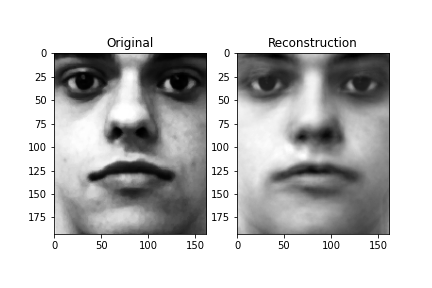
\includegraphics[width=0.40\textwidth]{../outputs/ans2/PCs_15.png}}
    \subfigure[20 PCs]{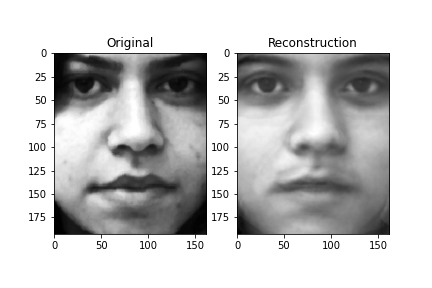
\includegraphics[width=0.40\textwidth]{../outputs/ans2/PCs_20.png}} \\
    \end{figure}
\begin{figure}
    \centering
    \subfigure[25 PCs]{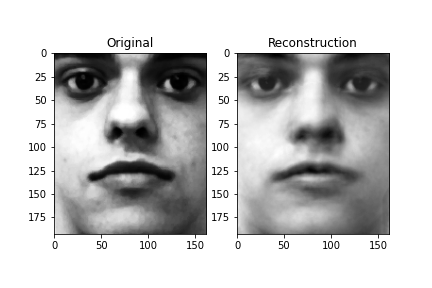
\includegraphics[width=0.40\textwidth]{../outputs/ans2/PCs_25.png}}
    \subfigure[40 PCs]{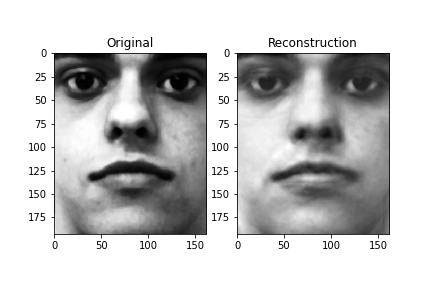
\includegraphics[width=0.40\textwidth]{../outputs/ans2/PCs_40.png}} \\
    \end{figure}
\begin{figure}
    \centering
    \subfigure[55 PCs]{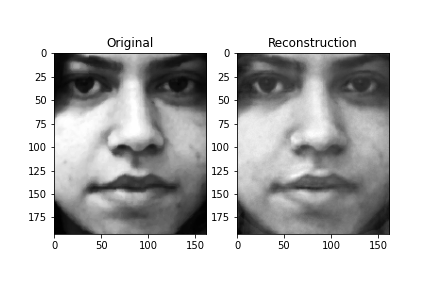
\includegraphics[width=0.40\textwidth]{../outputs/ans2/PCs_55.png}}
    \subfigure[70 PCs]{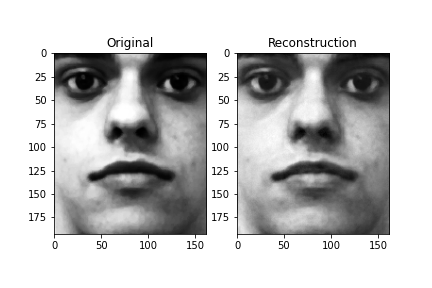
\includegraphics[width=0.40\textwidth]{../outputs/ans2/PCs_70.png}} \\
    \end{figure}
\begin{figure}
    \centering
    \subfigure[85 PCs]{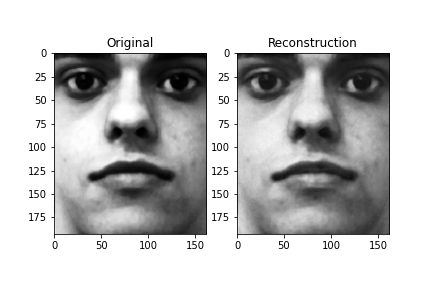
\includegraphics[width=0.4\textwidth]{../outputs/ans2/PCs_85.png}}
    \subfigure[100 PCs]{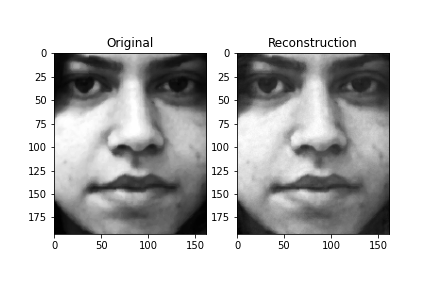
\includegraphics[width=0.4\textwidth]{../outputs/ans2/PCs_100.png}} \\
    \end{figure}
\begin{enumerate}
    [label=$\bullet$]
    \item We also see that there is no visible difference between image reconstructed using 100 PCs and original image. The MSE between these images is also almost 0. This is as expected since, this image in present in our training set. So, we can say that we have found fairly consistent basis for the image space.
\end{enumerate}
\section*{Problem 3}
\begin{figure}[htbp]
    \centering
    \subfigure[MSE vs Number of PCs]{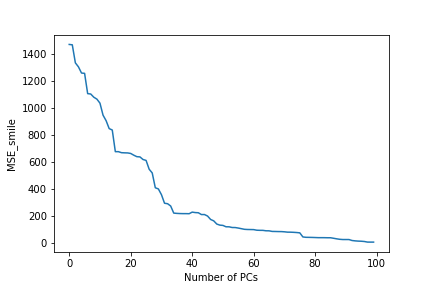
\includegraphics[width=0.50\textwidth]{../outputs/ans3/MSE_smile.png}}
    \end{figure}
\begin{enumerate}
    [label=$\bullet$]
    \item As we can see from the plot, initially MSE decreases drastically when we increase the number of PCs. After a certain number of PCs, the decrease in MSE is not so steep eventhough we increase the number of PCs. This is due to similar reason mentioned in the previous part. 
    \item The Principal Components, after about 25 most representative eigenfaces, does not provide substantial additional information to improve the reconstructed image drastically. This was also inferred by analysing corresponding eigenvalues in problem 1. 
    \item We also see that there is no visible difference between image reconstructed using 100 PCs and original image. The MSE between these images is also almost 0. This is as expected since, this image in present in our training set. So, we can say that we have found fairly consistent basis for the image space.
\end{enumerate}
\begin{figure}[htbp]
    \centering
    \subfigure[5 PCs]{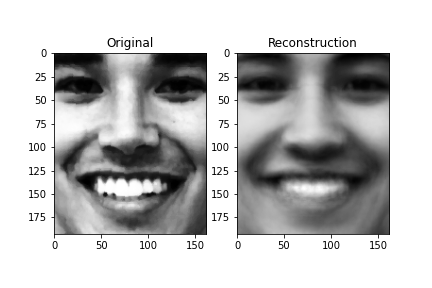
\includegraphics[width=0.3\textwidth]{../outputs/ans3/PCs_5.png}}
    \subfigure[10 PCs]{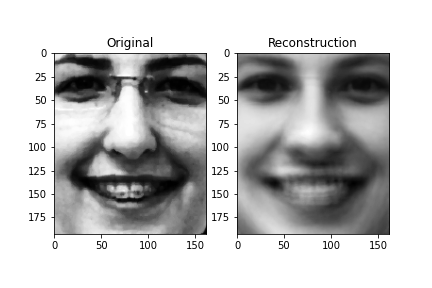
\includegraphics[width=0.3\textwidth]{../outputs/ans3/PCs_10.png}} \\
    \end{figure}
\begin{figure}
    \centering
    \subfigure[15 PCs]{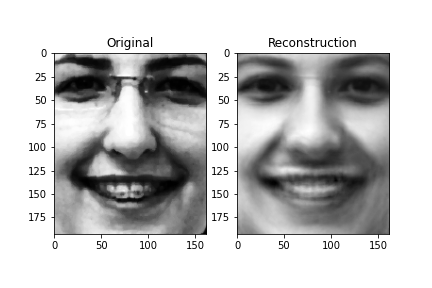
\includegraphics[width=0.3\textwidth]{../outputs/ans3/PCs_15.png}}
    \subfigure[20 PCs]{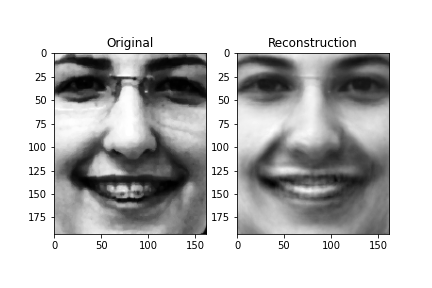
\includegraphics[width=0.3\textwidth]{../outputs/ans3/PCs_20.png}} \\
    \end{figure}
\begin{figure}
    \centering
    \subfigure[25 PCs]{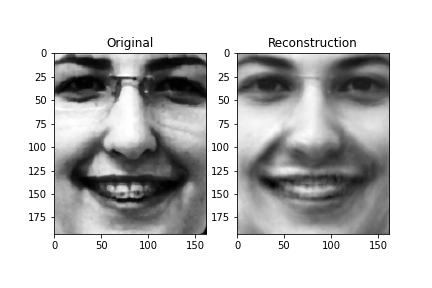
\includegraphics[width=0.3\textwidth]{../outputs/ans3/PCs_25.png}}
    \subfigure[40 PCs]{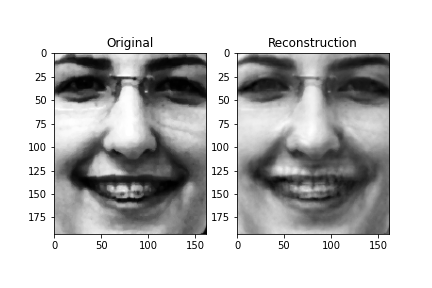
\includegraphics[width=0.3\textwidth]{../outputs/ans3/PCs_40.png}} \\
    \end{figure}
\begin{figure}
    \centering
    \subfigure[55 PCs]{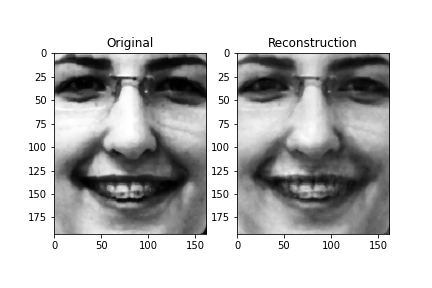
\includegraphics[width=0.3\textwidth]{../outputs/ans3/PCs_55.png}}
    \subfigure[70 PCs]{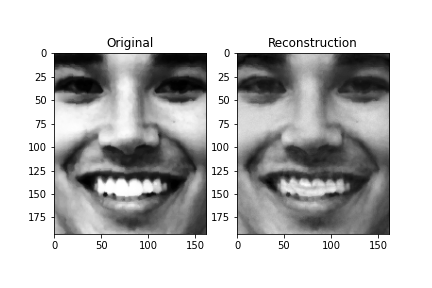
\includegraphics[width=0.3\textwidth]{../outputs/ans3/PCs_70.png}} \\
    \end{figure}
\begin{figure}
    \centering
    \subfigure[85 PCs]{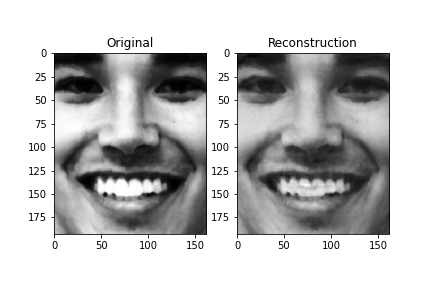
\includegraphics[width=0.3\textwidth]{../outputs/ans3/PCs_85.png}}
    \subfigure[100 PCs]{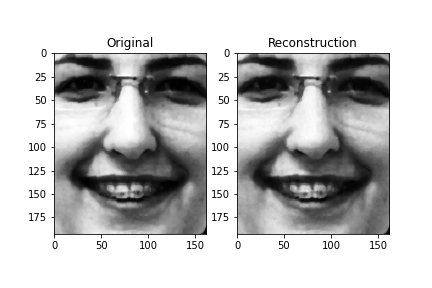
\includegraphics[width=0.3\textwidth]{../outputs/ans3/PCs_100.png}} \\
    \end{figure}
\section*{Problem 4}
\subsection*{Neutral}
\begin{enumerate}
    [label=$\bullet$]
    \item Since we are randomly sampling to generate the test and train set, we observe that MSE would not always be the same. After testing several times we see that variance in MSE is about 200 units. We can infer from above plot that behaviour of the algorithm does not change for the test set i.e. MSE decreases as we increase the number of Principal Components.
    \item Contrary to MSE from trainset image (minimum MSE = 0), we see that even after using all possible principal components (100), we still couldn't get MSE of testset image down to 0. Least MSE obtained was about 100 units. Since, MSE on testset image is never too low it is safe to say that we did not overfit the model, and the obtained model could be used for more general datapoints.
\end{enumerate}
\begin{figure}[htbp]
    \centering
    \includegraphics*[width=0.5\textwidth]{../outputs/ans4/MSE_test_neutral.png}
    \caption{MSE vs Number of PCs for Neutral Testset Image}
    \end{figure}
\begin{enumerate}
    [label=$\bullet$]
    \item On reconstructing the image, we see that the image is not as sharp as original image. We also observe that, the model atleast captured the key features appropriately, for example: contours of features of face (eyes, mouth, eyebrows). We can also see that there is vast difference in the shades of grayscale between the images.
    \item The image generated by our model is visually (perceived by us) the image of same face as the groundtruth face. In some cases, it visually (perceived by us) seems that we get better reconstructed image using lower PCs (Eg: 40) instead of 100 which is contrary to plotted MSE (since MSE decreases with increase in PCs).
    \item Model was also not always able to recreate the accessory (glasses) worn by the person in the image.
\end{enumerate}
\begin{figure}[htbp]
    \centering
    \subfigure[5 PCs]{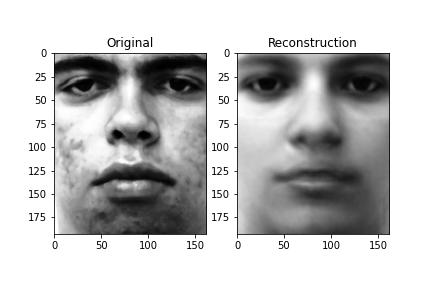
\includegraphics[width=0.3\textwidth]{../outputs/ans4/PCs_neutral_5.png}}
    \subfigure[10 PCs]{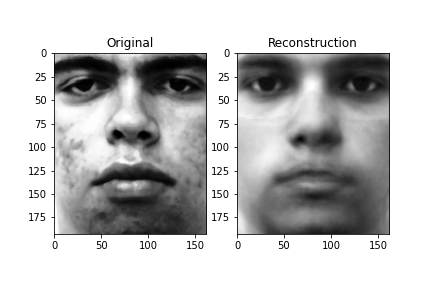
\includegraphics[width=0.3\textwidth]{../outputs/ans4/PCs_neutral_10.png}} \\
    \end{figure}
\begin{figure}
    \centering
    \subfigure[15 PCs]{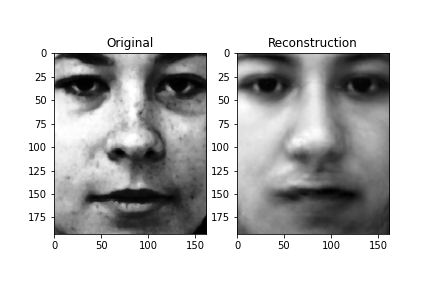
\includegraphics[width=0.3\textwidth]{../outputs/ans4/PCs_neutral_15.png}}
    \subfigure[20 PCs]{\includegraphics[width=0.3\textwidth]{../outputs/ans4/PCs_neutral_20.png}} \\
    \end{figure}
\begin{figure}
    \centering
    \subfigure[25 PCs]{\includegraphics[width=0.3\textwidth]{../outputs/ans4/PCs_neutral_25.png}}
    \subfigure[40 PCs]{\includegraphics[width=0.3\textwidth]{../outputs/ans4/PCs_neutral_40.png}} \\
    \end{figure}
\begin{figure}
    \centering
    \subfigure[55 PCs]{\includegraphics[width=0.3\textwidth]{../outputs/ans4/PCs_neutral_55.png}}
    \subfigure[70 PCs]{\includegraphics[width=0.3\textwidth]{../outputs/ans4/PCs_neutral_70.png}} \\
    \end{figure}
\begin{figure}
    \centering
    \subfigure[85 PCs]{\includegraphics[width=0.3\textwidth]{../outputs/ans4/PCs_neutral_85.png}}
    \subfigure[100 PCs]{\includegraphics[width=0.3\textwidth]{../outputs/ans4/PCs_neutral_100.png}} \\
    \end{figure}
\subsection*{Smiling}
\begin{enumerate}
    [label=$\bullet$]
    \item Since we are randomly sampling to generate the test and train set, we observe that MSE would not always be the same. After testing several times we see that variance in MSE is about 200 units. We can infer from above plot that behaviour of the algorithm does not change for the test set i.e. MSE decreases as we increase the number of Principal Components.
    \item Contrary to MSE from trainset image (minimum MSE = 0), we see that even after using all possible principal components (100), we still couldn't get MSE of testset image down to 0. Least MSE obtained was about 100 units. Since, MSE on testset image is never too low it is safe to say that we did not overfit the model, and the obtained model could be used for more general datapoints.
\end{enumerate}
\begin{figure}[htbp]
    \centering
    \includegraphics*[width=0.5\textwidth]{../outputs/ans4/MSE_test_smile.png}
    \caption{MSE vs Number of PCs for Smiling Testset Image}
    \end{figure}
\begin{enumerate}
    [label=$\bullet$]
    \item On reconstructing the image, we see that the image is not as sharp as original image. We also observe that, the model atleast captured the key features appropriately, for example: contours of features of face (eyes, mouth, smile, eyebrows). We can also see that there is vast difference in the shades of grayscale between the images.
    \item The image generated by our model is visually (perceived by us) the image of same face as the groundtruth face. In some cases, it visually (perceived by us) seems that we get better reconstructed image using lower PCs (Eg: 40) instead of 100 which is contrary to plotted MSE (since MSE decreases with increase in PCs).
    \item Model was also not always able to recreate the accessory (glasses) worn by the person in the image.
\end{enumerate}
\begin{figure}[htbp]
    \centering
    \subfigure[5 PCs]{\includegraphics[width=0.3\textwidth]{../outputs/ans4/PCs_smile_5.png}}
    \subfigure[10 PCs]{\includegraphics[width=0.3\textwidth]{../outputs/ans4/PCs_smile_10.png}} \\
    \subfigure[15 PCs]{\includegraphics[width=0.3\textwidth]{../outputs/ans4/PCs_smile_15.png}}
    \subfigure[20 PCs]{\includegraphics[width=0.3\textwidth]{../outputs/ans4/PCs_smile_20.png}}
    \end{figure}
\begin{figure}[htbp]
    \centering
    \subfigure[25 PCs]{\includegraphics[width=0.3\textwidth]{../outputs/ans4/PCs_smile_25.png}}
    \subfigure[40 PCs]{\includegraphics[width=0.3\textwidth]{../outputs/ans4/PCs_smile_40.png}}
    \subfigure[55 PCs]{\includegraphics[width=0.3\textwidth]{../outputs/ans4/PCs_smile_55.png}}\\
    \subfigure[70 PCs]{\includegraphics[width=0.3\textwidth]{../outputs/ans4/PCs_smile_70.png}}
    \subfigure[85 PCs]{\includegraphics[width=0.3\textwidth]{../outputs/ans4/PCs_smile_85.png}}
    \subfigure[100 PCs]{\includegraphics[width=0.3\textwidth]{../outputs/ans4/PCs_smile_100.png}}
    \end{figure}
\section*{Problem 5}
\begin{enumerate}
    [label=$\bullet$]
    \item Overall accuracy = 0.95
    \item Accuracy on Neutral Expression = 0.96875 (number of neutral images in testset = 32)
    \item Accuracy on Smiling Expression = 0.9285714285714286 (number of smiling images in testset = 28)
    \item The analysis (and above mentioned results) mentioned is with respect to the latest execution of the notebook. The core analysis should be the same, but as we are changing the sampling at every execution, there might be a few small variations with respect to the analysis.
\end{enumerate}
\subsection*{Possible Failures to algorithm}
\subsubsection*{Groundtruth: Neutral; Predicted: Smile}
\begin{enumerate}
    [label=$\bullet$]
    \item The algorithm fails because values of reconstructed smiling image at the mouth matches more accurately with original image (both are darker at the center of mouth compared to other regions) compared to reconstructed neutral expression image. 
    \item This could mainly happen due to difference in lighting while capturing the images, which would wide range of values in the array for both expressions. One other factor which could cause error is different people have different smiling and neutral expression. 
    \item So, when there is visually (perceived by us) not much difference in the neutral and smiling expressions of a person, the model might also have a hard time in predicting the expression accurately (For example: the shape of lips while smiling and neutral might be same or not much difference in the smiling and neutral faces).
\end{enumerate}
\subsubsection*{Groundtruth: Smile; Predicted: Neutral}
\begin{enumerate}
    [label=$\bullet$]
    \item The algorithm fails because values of reconstructed neutral image at the mouth matches more accurately with original image (both are lighter at the center of mouth compared to other regions) compared to reconstructed smiling expression image. 
    \item This could mainly happen due to difference in lighting while capturing the images, which would wide range of values in the array for both expressions. One other factor which could cause error is different people have different smiling and neutral expression. 
    \item So, when there is visually not much difference in the neutral and smiling expressions of a person, the model might also have a hard time in predicting the expression accurately (For example: the shape of lips while smiling and neutral might be same or not much difference in the smiling and neutral faces).
\end{enumerate}
\newpage
\subsubsection*{Results}
\begin{figure}[htbp]
    \centering
    \subfigure[Truth:0; Mislabel: 1]{\includegraphics[width=0.3\textwidth]{../outputs/ans5/mislabel_0.png}}
    \subfigure[Truth:0; Mislabel: 1]{\includegraphics[width=0.3\textwidth]{../outputs/ans5/mislabel_1.png}}
    \subfigure[Truth:1; Mislabel: 0]{\includegraphics[width=0.3\textwidth]{../outputs/ans5/mislabel_2.png}}    
    \caption{Mislabelled Images}
\end{figure}
\newpage
\subsubsection*{Possible Solutions}
\begin{enumerate}
    [label=$\bullet$]
    \item We could increase the number of Principal Components to obtain more accurate reconstructed images. Also, while collecting the dataset we could increase the variation of lighting in the trainset, so that we don't encounter such an error while testing. 
    \item One other variation could be including both types of faces in the training set, i.e. people whose smile and neutral face differ prominently and people whose smile and neutral face is similar.
\end{enumerate}
\section*{References}
\begin{enumerate}
    \item \href{http://www.mit.edu/~9.54/fall14/Classes/class10/Turk%20Pentland%20Eigenfaces.pdf}{Face Recognition Using Eigenfaces by Matthew Turk and Alex Pentland; Vision and Modeling Group, MIT Media Laboratory}
    \item \href{https://watermark.silverchair.com/jocn.1991.3.1.71.pdf?token=AQECAHi208BE49Ooan9kkhW_Ercy7Dm3ZL_9Cf3qfKAc485ysgAAAtcwggLTBgkqhkiG9w0BBwagggLEMIICwAIBADCCArkGCSqGSIb3DQEHATAeBglghkgBZQMEAS4wEQQMVF3omRZLNx56gCwzAgEQgIICijPdO1SlMn02mQrnVwR1OjQF68H9DKArXsQJbkvyM-5-Vb-ZyV_CZjtkmPACKF1xLBd7QCjLz9_I1YaaKpu0okVXPQiFYzfcH-I5ZJNjiaMxinGwSZ1Cf_S7TZBxkiyKi5ok3NGXtGfCvfHHByqXlx1k48ewccqNHa-VjqlW-8gf_ePErjzpfGZ2MQlu-sYVwTGUTExYdnx3PkuLeHeNbqahxmela8LNzvEBCEEY-2dgFzIPROrHqOXlohAGnmf4KTsGaYhMa8gNeKvAQ-5O-9MkS1daqSs9RDV3Km3d9_o2Uakrie0RDzNN5FeMVb4KtC_MiYS6c9yFqEDI6EFrTubgjaRd_rt21JHE1auXlcWMDY2GhDh4az9F_DuZF3bWpldjHdCND0kqRm6rKEuzbai8VjzP4gJVY8LawvlMTg9xs2VboB58krvblWqyUO9iISg7OLYyCfxPbWe1G8EM1-YoOwZ-egbAu4gDOtlkSseO8eME4ib3IdANQ6xnDumbiUxZHXF02KecKu8QF1sw_dxqf0Y7LforT9fvsr9eBa0sFOJVBStHjOXm2mtqaCS-CJ9JaTwJxVqyn0FAQOOyZ4gqLvfxaCw2rW89y4YxsXnERLJ9eETlaNHGe8M1-tXOpxPRl-MaNXVYI_MFxUwoFW2KOF1VhUQB4A0SteT6FLQ_aac-_2bl1AlSCqpRVVaZzDzgMWmgxw-6NGaptMGtjD7_KTqPB4bZbrt4qQDDJTzZk1QKmkTNixnsbOpFEZW26aY34GelXf-OfVvwLUu9drXDdT8qDCvye9hvrpuivKBYHRceOlSjfYNejnLp5MKrRvQp6ESAvmPgeRDJV0GJ0JDd6DcJFkztRs_m}{Eigenfaces for Recognition by Matthew Turk and Alex Pentland}
\end{enumerate}
\end{document}